\section{Полученные результаты}

\subsection{Слова, где $ L(S) > Z(S) $}

С помощью перебора, описанного в предыдущем разделе, были проверены все бинарные слова длиной до 34 символов включительно. Оказалось, что самое короткое слово с данным свойством имеет длину 14. На проверенных длинах разность $ L(S) - Z(S) $ не превысила 2. Таблицы с кратчайшими словами, где $ L(S) > Z(S) $, и их количеством представлены в приложении A.

Список всех найденных слов с данным свойством доступен по ссылке: \linebreak
\url{https://raw.githubusercontent.com/borzunov/course-work-2016/master/bruteforce/result.txt}

Простого закона для зависимости кол-ва слов длины $n$ с данным свойством от числа $n$ (рис. 1 ниже) найдено не было. По графику на рис. 2 можно предположить, что доля слов с данным свойством среди всех слов определённой длины стремится к нулю.

\begin{figure}[h!]
\begin{center}
\begin{minipage}[h]{0.49\linewidth}
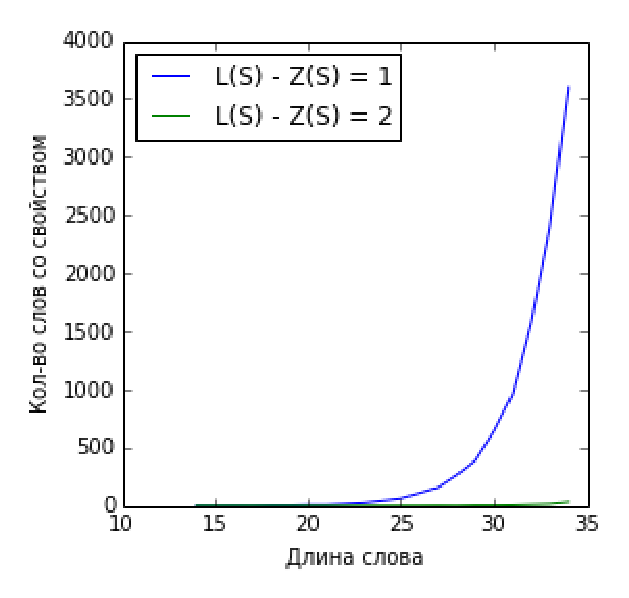
\includegraphics[width=1\linewidth]{word_count}
\caption{Кол-во слов с указанными свойствами.}
\label{pic:word_count}
\end{minipage}
\hfill 
\begin{minipage}[h]{0.49\linewidth}
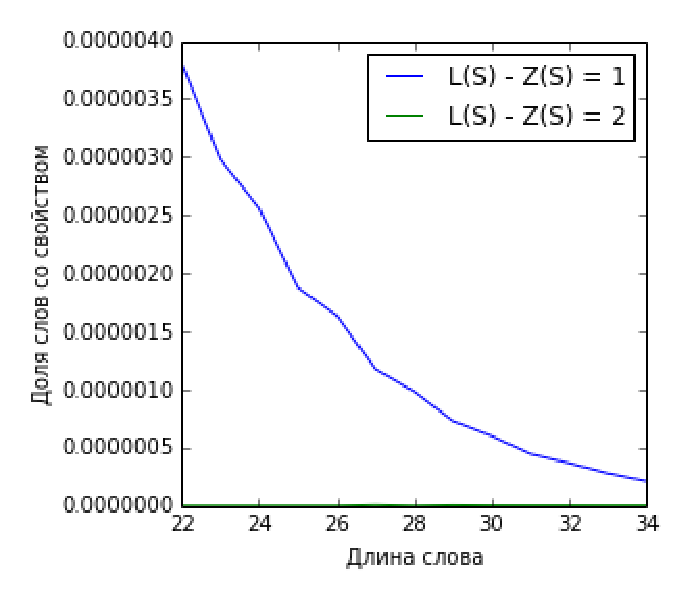
\includegraphics[width=1\linewidth]{word_fraction}
\caption{Доля слов с указанными свойствами среди всех слов заданной длины.}
\label{pic:word_fraction}
\end{minipage}
\end{center}
\end{figure}

\subsection{Построенные серии строк}

После поиска закономерностей в кратчайших словах с заданным свойством по аналогии были построены несколько серий строк, где $ L(S) $ существенно превышает $ Z(S) $. Тем не менее, во всех сериях не нарушается гипотеза о том, что $ L(S) = O( Z(S) ) $. Серии перечислены ниже:

\begin{enumerate}

\item
    $$ S_n = \prod_{i = n}^{1} (10)^i 0 $$
    
    Для $ n = 2 k $ имеем:
    $$ L(S_n) = 2 k + 2 \qquad Z(S_n) = k + 3 \qquad \frac{L(S_n)}{Z(S_n)} \to 2 $$
    
    Пример для $ n = 6 $:
    
    \begin{itemize}
    \item
        Слово:
        
        \texttt{101010101010 0 1010101010 0 10101010 0 101010 0 1010 0 10 0}
    \item
        Разбиение Линдона (8 различных сегментов):
        
        \texttt{1 01 01 01 01 01 00101010101 001010101 0010101 00101 001 0 0}
    \item
        Разбиение Лемпеля-Зива (6 сегментов):
        
        \texttt{1 0 1010101010 01010101010010101010 010101001010 0100}
    \end{itemize}
    
    Похожая серия с чуть более сложной формулой при $ n = 2 $ даёт слово наименьшей длины, у которого $ L(S) > Z(S) $:
    
    $$ S_n = \left ( \prod_{i = n + 1}^{2} (10)^i 0 \right ) \cdot 10 $$
    
    Упомянутое слово имеет длину 14:
    
    \begin{itemize}
    \item
        Слово:
        
        \texttt{101010 0 1010 0 10}
    \item
        Разбиение Линдона (5 различных сегментов):
        
        \texttt{1 01 01 00101 001 0}
    \item
        Разбиение Лемпеля-Зива (4 сегмента):
        
        \texttt{1 0 1010 01010010}
    \end{itemize}
    
\item
    $$ S_n = \prod_{k = n}^{1} \prod_{i = k}^{1} (10)^i 0 $$
    
    Для $ n = 2 k $ имеем:
    $$ L(S_n) = 4 k \qquad Z(S_n) = 3 k \qquad \frac{L(S_n)}{Z(S_n)} = \frac{4}{3} $$
    
    Пример для $ n = 4 $:
    
    \begin{itemize}
    \item
        Слово:
        
        \texttt{10101010 0 101010 0 10100 10 0 \quad 101010 0 1010 0 10 0 \quad 1010 0 10 0 \quad 10 0}
    \item
        Разбиение Линдона (8 различных сегментов):
        
        \texttt{1 01 01 01 0010101 00101 001001010100101 00100101 001 001 0 0}
    \item
        Разбиение Лемпеля-Зива (6 сегментов):
        
        \texttt{1 0 101010 010101001010 01001010100101001001010 0100100}
    \end{itemize}

\item
    $$ S_n = \prod_{k = n}^{1} \prod_{j = k}^{1} \prod_{i = j}^{1} (10)^i 0 $$
    
    Для $ n = 2 k $ имеем:
    $$ L(S_n) = 6 k - 2 \qquad Z(S_n) = 5 k - 3 \qquad \frac{L(S_n)}{Z(S_n)} \to \frac{6}{5} $$
    
    Пример для $ n = 4 $:
    
    \begin{itemize}
    \item
        Слово:
        
        \texttt{1010101001010100101001001010100101001001010010010010101001010010010100}
        
        \texttt{10010010100100100100}
    \item
        Разбиение Линдона (10 различных сегментов):
        
        \texttt{1 01 01 01 0010101 00101 001001010100101 00100101}
        
        \texttt{00100100101010010100100101 00100100101 001 001 001 0 0}
    \item
        Разбиение Лемпеля-Зива (7 сегментов):
        
        \texttt{1 0 101010 010101001010 01001010100101001001010}
        
        \texttt{0100100101010010100100101001001001010 0100100100}
    \end{itemize}
    
\item
    Аналогично предыдущим сериям, можно составить:
    $$ S_n = \prod_{m = n}^{1} \prod_{k = m}^{1} \prod_{j = k}^{1} \prod_{i = j}^{1} (10)^i 0 $$
    
    Для $ n = 2 k $ имеем:
    $$ L(S_n) = 8 k - 4 \qquad Z(S_n) = 7 k - 6 \qquad \frac{L(S_n)}{Z(S_n)} \to \frac{8}{7} $$

\end{enumerate}
